% ED-09 -- The bilayer dipolar-exciton interaction is completely monotone
% Sources: TOP20.json pick 9; papers/ar_dipolar_exciton/{AUDIT.md,REVISION.md,publication_meta.json,gen_numbers.tex,
%          data/lattice_gaps.jsonl}
% Figure: code/fig09.py -> figures/c09_dipoles.{pdf,png}
\chapter[Des excitons en triangles]{Des paires électron--trou qui se rangent en triangles, sur le papier}
\reference{Préprint du 25 octobre 2026.\\ doi:10.5281/\\zenodo.23646103}

\section*{L'idée en une image}

\begin{analogie}
Une garantie existe déjà~: \og toute recette dont les ingrédients respectent tel cahier des charges donne un plat
réussi\fg. On ne refait pas la garantie~; on prend un ingrédient nouveau, on vérifie point par point qu'il respecte
le cahier des charges, et la garantie s'applique alors à lui. Ici, la garantie est le théorème du réseau
triangulaire issu du dépôt openai/math, le cahier des charges est la propriété dite \og complètement monotone\fg, et
l'ingrédient nouveau est la répulsion entre deux excitons dans un empilement de deux couches atomiques.

\emph{Où l'image cesse d'être juste~:} la garantie elle-même n'a pas été relue par des pairs, et elle porte sur des
particules classiques immobiles au zéro absolu~; de vrais excitons, à ces densités, forment un gaz quantique.
\end{analogie}

\section*{Ce qui a été fait}

Un exciton est une paire liée d'un électron et d'un \og trou\fg{} (une absence d'électron, de charge positive).
Quand l'électron vit dans une couche et le trou dans la couche voisine, à la distance $d$, la paire devient un
petit dipôle vertical. Deux tels dipôles, à la distance $r$ dans le plan, se repoussent~: les deux électrons se
repoussent, les deux trous aussi (deux termes $1/r$), et chaque électron attire le trou de l'autre à travers
l'intervalle (deux termes $1/\sqrt{r^2+d^2}$). Bilan~:
\[
V(r)=2\Bigl(\frac1r-\frac1{\sqrt{r^2+d^2}}\Bigr).
\]
L'article démontre dans Lean que cette répulsion, vue comme fonction du carré de la distance $t=r^2$, a la
propriété exigée par le théorème amont~: elle est positive, elle décroît, sa pente s'aplatit, et ainsi de suite
avec des signes qui alternent à tous les ordres de dérivation. Il en déduit que le réseau triangulaire a la plus
petite énergie parmi toutes les configurations, \emph{à toutes les densités}, et que cette énergie est finie (sans
quoi l'inégalité ne dirait rien d'utile).

\begin{encadre}
\textbf{À faire avec un crayon.} Prenez $d=1$.
\begin{itemize}
\item À la distance $r=1$~: $V=2(1-1/\sqrt2)=2-\sqrt2\approx0{,}586$.
\item À la distance $r=10$~: $V=2(0{,}1-1/\sqrt{101})\approx2(0{,}1-0{,}099504)\approx0{,}000993$, presque exactement
  $d^2/r^3=0{,}001$. De loin, la paire se comporte comme un dipôle (figure~\ref{fig:c09}, à gauche).
\item Les signes, en $t=1$ avec $d^2=3$~: $g(t)=2(t^{-1/2}-(t+3)^{-1/2})$ vaut $2(1-\tfrac12)=1>0$~; sa dérivée vaut
  $-(1-\tfrac18)=-\tfrac78<0$~; sa dérivée seconde vaut $\tfrac32(1-\tfrac1{32})=\tfrac{93}{64}>0$. Les signes
  alternent, comme le demande le cahier des charges.
\item Contre-épreuve~: avec un décalage négatif, $t^{-1/2}-(t-c)^{-1/2}$ ($c>0$) est \emph{négatif}~; la propriété
  tombe, et Lean le démontre aussi.
\end{itemize}
\end{encadre}

\begin{figure}[htbp]
\centering
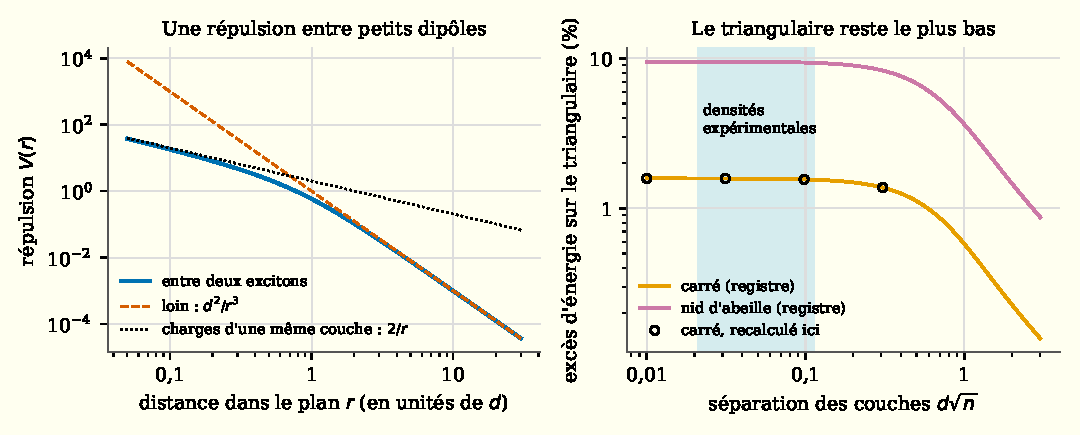
\includegraphics[width=\linewidth]{figures/c09_dipoles}
\caption{La répulsion entre dipôles (gauche)~; excès d'énergie des réseaux carré et nid d'abeille (droite, \niveau{X}).}
\label{fig:c09}
\end{figure}

\section*{Comment on s'est assuré que ce n'est pas faux}

En résumé~: \niveau{A} pour l'admissibilité et les corollaires (conditionnels au théorème amont), \niveau{C} pour la
lecture physique, \niveau{X} pour les simulations.

Pour les énoncés Lean, \og le juge a regardé\fg~: le noyau de Lean (le petit programme qui contrôle chaque pas logique) a accepté les
démonstrations, avec seulement trois axiomes standard. Un auditeur séparé, un agent d'IA distinct, a
recompilé les modules depuis les sources et planté ses propres fausses preuves (un trou \texttt{sorry}, un axiome
inventé)~: toutes deux ont été dénoncées. Les modules ont été rejoués dans le noyau le 26 octobre 2026 sans erreur.

Côté calcul, une esquisse au crayon, un module Rust du solveur rusty-SUNDIALS a calculé les énergies exactes des
réseaux, et l'auditeur les a retrouvées par une méthode toute différente, à environ $10^{-13}$ près. Des relaxations
préenregistrées n'ont trouvé aucune configuration périodique sous le réseau triangulaire (0 sur 21)~; l'article
précise honnêtement que 7 de ces 21 essais étaient des contre-épreuves conçues pour rester au-dessus, que deux
essais finissent dans le même état, et que le calcul d'énergie a changé de méthode par rapport au plan annoncé. Le
registre reste marqué \og non audité\fg~: aucun humain n'a relu les énoncés.

\section*{Ce que ça ne dit pas}

\begin{limite}
\begin{itemize}
\item Tout est \emph{conditionnel} au théorème amont, généré par une IA et non relu par des pairs.
\item Le modèle est classique, au zéro absolu, avec des dipôles rigides et sans écrantage. Avec des écartements de
  couches d'environ $6{,}6$~Å, tirés d'une base de données publique, les écarts d'énergie entre réseau carré et
  triangulaire ne valent que $0{,}0014$ à $0{,}22$~meV par exciton~: environ 1,5 à 5 ordres de grandeur sous la
  profondeur des pièges de moiré cités dans la littérature (des dizaines à une centaine de meV). Rien n'annonce donc qu'on verra ces
  triangles au laboratoire.
\item La finitude de l'énergie n'est démontrée que pour cette répulsion, pas pour toute la famille voisine.
\item La complète monotonie est élémentaire~; la nouveauté est modeste~: c'est le corollaire vérifié.
\end{itemize}
\end{limite}

\section*{Pour aller plus loin}

L'article, son registre et l'audit sont déposés sous doi:10.5281/\allowbreak zenodo.23646103. La même démarche a été appliquée
à la force qui règne dans une monocouche (doi:10.5281/zenodo.23646107).
